\subsection{Sprint 9: da 2024-07-11 a 2024-07-20}
\par Il team ha completato la struttura per presentarsi alla \glossario{RTB}, gli sforzi del gruppo di concentreranno sull’aggiornamento e la revisione della documentazione prodotta fino allo sprint corrente..

\subsubsection{Obiettivi}
\begin{itemize}
  \item Presentazione e consegna \glossario{RTB};
  \item Espansione delle \NdP\ nelle seguenti sezioni:
  \begin{itemize}
    \item Sviluppo;
    \item Verifica;
    \item Validazione;
    \item Strumenti;
  \end{itemize}
  \item Suddivisione delle metriche in base all’obiettivo;
  \item Aggiornamento dei grafici nel cruscotto di valutazione della qualità;
  \item Revisione delle metriche di processo e di prodotto;
  \item Inizio stesura Specifica tecnica.
\end{itemize}

\begin{figure}[H]
  \centering
  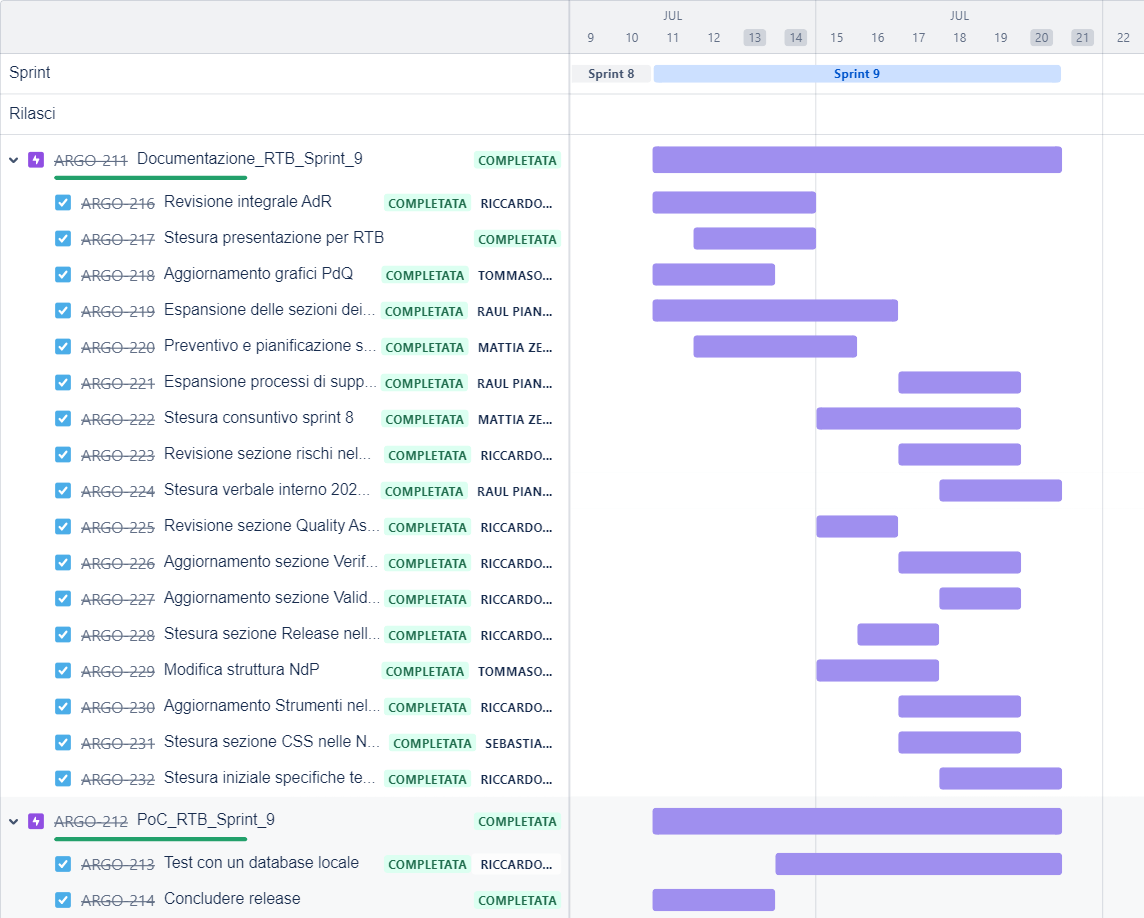
\includegraphics[width=0.90\textwidth]{assets/Pianificazione/Sprint-9/gantt.png}
  \caption{Sprint 9 - Diagramma di Gantt}\label{fig:sprint-9-gantt}
\end{figure}

